\chapter{Training a Convolutional Neural Network}
Once the network has been constructed the user needs to tune the hyperparameters in order to get the best loss and learning rate from their network in the shortest possible time. This is the most time consuming part of the process as there are many different parts of the network that can be adjusted to produce different results. The three hyperparameters that need to be adjusted are as follows:
\begin{itemize}
    \item The number of filters in the convolutional layers
    \item The batch size
    \item The optimiser and the learning rate for said optimiser.
\end{itemize}
These will be discussed further in this chapter. There are other hyperparameters that can be adjusted but considering the time and resources available this was not possible within the scope of this thesis. This thesis chose to use a simple grid search to determine which was the most optimal hyperparameter combination. Studies have shows that random search reduces the amount of time required to find the most optimal hyperparameters (\cite{bergstra12}). Building upon random search, there is a new technique that uses bayesian optimisation (\cite{snoek12}) to search for the best combination of hyperparameters.
\par
At the end of this chapter there will be a brief discussion about the other hyperparameters that could have been adjusted that were not within the scope of this study. 
\section{Hyperparameter Optimisation}
The aim of hyperparameter optimisation is to find the combination of hyperparameters that produce the lowest loss for our model. We have built our model that has a learning alorithm with defined parameters. However, the learning algorithm also comes with bells and whistles that need to be defined before the learning algorithm can be run (\cite{bergstra12}), these are known as hyperparameters ($\lambda$). Once $\lambda$ is defined, the model is run and the results evaluated, this is repeated until a $\lambda$ is chosen that produces the lowest loss. 
\subsection{Grid Search}
Grid search (\cite{lecun10,larochelle07}) is the most widely used method for hyperparameter tuning. The user defines a set of discrete values for each hyperparameter they would like to adjust after each iteration. Then, by fixing one and varying the others, the hyperparameters are changed and evaluated throughout training. This method was used here as it is simplest to implement. The disadvantage of using grid search is that all hyperparameters are given equal importance so too much time is spent exploring dimensions that do not matter (\cite{bergstra12}). This method suffers from what is known as the \textit{curse of dimensionality} as increasing the number of hyperparameters causes the number of trials required to grow exponentially.
\begin{figure}
    \centering
    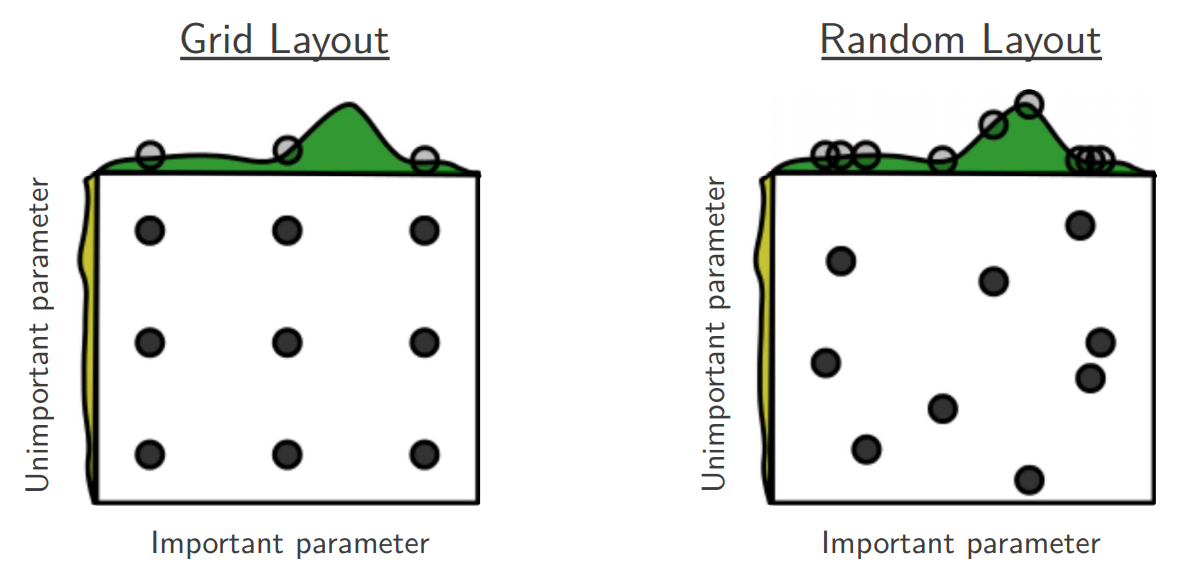
\includegraphics[width=\textwidth]{\dir/figs/grid_random.PNG}
    \caption[Grid Search versus Random Search]{The green part of the figure represents a the function used to evaluate the model. Grid search evaluates at three distinct parts of the function, potentially missing the most optimal combination. Whereas, random search evaluates all parts of the function randomly and is more likely to find the optimum combination. Taken from \citet{bergstra12}.}
    \label{fig.grid_random}
\end{figure}
\subsection{Random Search}
To implement random search the user defines the upper and lower bounds for the hyperparameters and the algorithm randomly selects a combination to be tested. \citet{bergstra12} empirically shows that this method is more efficient than grid search for low dimensional problems, this is shown in Figure \ref{fig.grid_random}. In most cases the loss function will be more sensitive to change in some dimension than others (see \cite{caflisch97}). For example, in most CNNs the learning rate is the most important hyperparameters but it is necessary to explore the other dimensions as well. If the user knew which dimensions were more important, a different grid search could be created to explore the more important dimension. To create a grid with enough detail to generalise the hyperparameters search for all datasets, will therefore be inefficient on an individual dataset basis due to the curse of dimensionality. For every irrelevant search dimension that is explored, there is an exponential number of grid search trials required (\cite{bergstra12}). It is in these conditions that random search thrives as it has the same efficiency while searching all the dimensions that it would have had if only searching the relevant ones.
\par
A few of the significant advantages that random search has over grid search are: random search can be stopped at any time and the completed trials represent a complete experiment; if more resources become available, new trials can be added; and every trial can be carried out asynchronously. 
\par
Bayesian optimisation methods offer principled approaches to weight the importance of each dimension (\cite{bergstra12}) and will be discussed in the next section.
\subsection{Bayesian Optimisation}
Bayesian optimisation (BO) (\cite{mockus78}) differs from random search and grid search because each hyperparameter selection is based on the previous model runs. Bayesian optimisation assumes that the unknown function being evaluated was a sample from a Gaussian process. The results of adjusting the hyperparameters on the distribution can then be observed (\cite{snoek12}). To pick the next hyperparameter combination, one can model the expected improvement over the current best result.
\par
CNNs differ from other optimisation problems because different hyperparameter combinations take different amounts of tine. For example, using fewer filters will take less time than more filters. Standard BO is subptimal when running jobs in parallel and so \citet{snoek12} have proposed a new BO algorithm that takes into account the variuability of the cost of certain combinations as well as the possibility of multiple processors being available. 
\par
BO is interested in finding the minimum of some function $f(x)$, within some domain of the hyperparameters $\chi$. BO works to construct a probabilistic model for $f(x)$ and exploits this model to make a decision about where in $\chi$ to next evaluate, while integrating out the uncertainty (\cite{brochu10, snoek12}). \par
A good search function finds the optimal hyperparameter combination in the shortest time available. \citet{snoek12} models the cost function $\ln c (x)$ alongside $f(x)$. Then the optimiser can easily compare the predicted duration and use it to calculate the expected improvement as a function of x.
\par
\citet{snoek12} also proposes the use of Monte Carlo estimates of the pending function evaluations to judge which hyperparameter combination to evaluate next. This allows the optimisation to work even when jobs are being run in parallel and there are no results from some of the combinations.
\paragraph{}
On the next iteration of this project, random search will be implemented to return the optimal hyperparameter combination through the least resource intensive path. Ultimately, this project would have been greatly improved if Bayesian optimisation had been implemented from the beginning as it would have resulted in a more robust methodology to evaluate the results of model training and find the optimal combination. 
\section{Hyperparameters}
\subsection{Number of Filters}
The convolution depth determines the architecture of the neural network. The user has to decide what value to start with as this dictates how deep the output of the final convolutional layer will be. This variable was mentioned in Section \ref{sub.CNN}, where \texttt{self.cr} was the number of filters to be determined by the user. Most CNNs tend to use numbers that are a power of 2 for all stages of implementation, as we can see from Figure \ref{fig.filter_size}, larger filters result in generally lower losses for our data. 
\begin{figure}[htbp]
\centering
\begin{subfigure}{0.45\textwidth}
\includegraphics[width=\textwidth]{\dir/figs/arch/{batch128lr0.01arch2epochs100}.png}
\caption{}
\label{fig.filter2}
\end{subfigure}%
\hfill
\begin{subfigure}{0.45\textwidth}
\includegraphics[width=\textwidth]{\dir/figs/arch/{batch128lr0.01arch4epochs100}.png}
\caption{}
\label{fig.filter4}
\end{subfigure}
\bigskip
\begin{subfigure}{0.45\textwidth}
\includegraphics[width=\textwidth]{\dir/figs/arch/{batch128lr0.01arch8epochs100}.png}
\caption{}
\label{fig.filter8}
\end{subfigure}
\hfill
\begin{subfigure}{0.45\textwidth}
\includegraphics[width=\textwidth]{\dir/figs/arch/{batch128lr0.01arch16epochs100}.png}
\caption{}
\label{fig.filter16}
\end{subfigure}
\bigskip
\begin{subfigure}{0.45\textwidth}
\includegraphics[width=\textwidth]{\dir/figs/arch/{batch128lr0.01arch32epochs100}.png}
\caption{}
\label{fig.filter32}
\end{subfigure}
\hfill
\begin{subfigure}{0.45\textwidth}
\includegraphics[width=\textwidth]{\dir/figs/arch/{batch128lr0.01arch64epochs100}.png}
\caption{}
\label{fig.filter64}
\end{subfigure}
\caption[Effect of adjusting the filter size on Loss of network]{Learning rate increases by a factor of two from two filters up to 64 filters. The dashed line displays the loss smoothed using a moving window of size calculating the average loss. (d) has a filter size of 32 and the loss here is generally smaller than in the other examples.}
\label{fig.filter_size}
\end{figure}
\subsection{Batch Size}
The batch size changes the size of the stack of data that is being fed into the neural network. A batch size of 1 will show a large fluctuation on the loss compared to a batch size the encompasses the whole dataset. A batch size that is the same size as the dataset should have small fluctuations in the loss unless the learning rate is too high. This is likely the case for the examples given in Figure \ref{fig.batch_size}
\begin{figure}[htbp]
\centering
\begin{subfigure}{0.45\textwidth}
\includegraphics[width=\textwidth]{\dir/figs/batch/{batch16lr0.01arch16epochs100}.png}
\caption{}
\label{fig.br18}
\end{subfigure}%
\hfill
\begin{subfigure}{0.45\textwidth}
\includegraphics[width=\textwidth]{\dir/figs/batch/{batch32lr0.01arch16epochs100}.png}
\caption{}
\label{fig.br32}
\end{subfigure}
\bigskip
\begin{subfigure}{0.45\textwidth}
\includegraphics[width=\textwidth]{\dir/figs/batch/{batch64lr0.01arch16epochs100}.png}
\caption{}
\label{fig.br64}
\end{subfigure}
\hfill
\begin{subfigure}{0.45\textwidth}
\includegraphics[width=\textwidth]{\dir/figs/batch/{batch128lr0.01arch16epochs100}.png}
\caption{}
\label{fig.br128}
\end{subfigure}
\caption[Effect of adjusting the batch size on Loss of network]{All four graphs show how adjusting the batch size rate effects the loss rate of the network after each epoch. (d) The largest batch size shows consistently the lowest loss.}
\label{fig.batch_size}
\end{figure}
\subsection{Learning Rate and Optimizer}
Optimisation works by finding the shortest path to the set of weights and biases that produce the lowest loss. If we consider our loss as a landscape, there will be peaks and troughs but ultimately a deepest point as shown in Figure \ref{fig.loss_landscape}. This deepest point is where the weights and biases have produced the lowest loss, searching for the quickest route to the deepest point is known as gradient descent.
\begin{figure}[htbp]
    \centering
    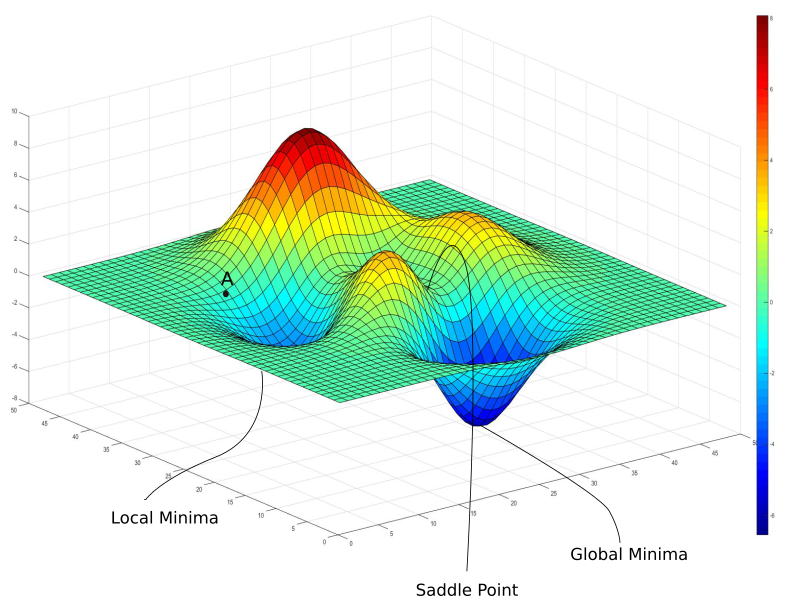
\includegraphics[width=0.8\textwidth]{\dir/figs/challenges-1.png}
    \caption[3D Schematic of CNN Loss]{Loss of the network is displayed as a 2D surface in 3D space. The  two issues that can prevent optimisation are labelled. Low loss is represented in blue and a high loss is represented as red. Taken from \citet{kathuria18}}
    \label{fig.loss_landscape}
\end{figure}
\par
The standard gradient descent algorithm for deep learning and CNNs is Stochastic Gradient Descent (SGD) (\cite{robbins51}). It is one of the most used training algorithms that despite it simplicity performs empirically well across a variety of applications. SGD has trouble navigating local minima (Figure \ref{fig.loss_landscape}), and will oscillate around the slopes and not converge on a loss. If we consider the optimisation as a ball starting from A in Figure \ref{fig.loss_landscape}, as it moves down towards the local minima, the ball gains inertia. SGD is improved by using a momentum method that simulates inertia so the function can escape local minima and saddle points to find the global minima of loss (\cite{ruder16}). 
\par
This project has focused on a variation of SGD with momentum known as the \textit{Adam} optimiser (\cite{kingma14}). This is one of a group of algorithms known as adaptive gradient descent algorithms as they dynamically adjust their parameters as training progresses depending on what has happened in the past. The \textit{Adam} optimiser updates the learning rate at each step as well as using momentum to make sure the optimiser does not oscillate within a local minima or on a saddle point. 
\par
It has been shown that when using sparse datasets it is more effective to use an adaptive algorithm as it allows for an initially high learning rate to be used as it will reduce as training progresses. \citet{kingma14} showed that the \textit{Adam} optimiser preformed the best out of the other adaptive gradient descent algorithms and is what has been used for this project. 
  \begin{figure}[htbp]
\centering
\begin{subfigure}{0.45\textwidth}
\includegraphics[width=\textwidth]{\dir/figs/lr/{batch128lr0.0001arch16epochs100}.png}
\caption{}
\label{fig.lr0.0001l}
\end{subfigure}%
\hfill
\begin{subfigure}{0.45\textwidth}
\includegraphics[width=\textwidth]{\dir/figs/lr/{batch128lr0.001arch16epochs100}.png}
\caption{}
\label{fig.lr0.001}
\end{subfigure}
\bigskip
\begin{subfigure}{0.45\textwidth}
\includegraphics[width=\textwidth]{\dir/figs/lr/{batch128lr0.01arch16epochs100}.png}
\caption{}
\label{fig.lr0.01}
\end{subfigure}
\hfill
\begin{subfigure}{0.45\textwidth}
\includegraphics[width=\textwidth]{\dir/figs/lr/{batch128lr0.1arch16epochs100}.png}
\caption{}
\label{fig.lr0.1}
\end{subfigure}
\caption[Effect of adjusting learning rate on Loss of network]{All four graphs show how adjusting the learning rate of the optimiser effects the loss rate of the network after each epoch. (b) returns the lowest loss, however there are large fluctuations in the returned loss..}
\label{fig.learning_rate}
\end{figure}

\section{Testing the Network}